\documentclass[aps,prl,reprint]{revtex4-1}
\usepackage{blindtext}

\usepackage{amsmath}
\usepackage{graphicx}
\usepackage{commath}
\usepackage{siunitx}
\usepackage{tabularx}
\usepackage{subcaption}

\usepackage{amssymb}

\usepackage{float}

\usepackage{graphicx}


\usepackage[b]{esvect}


\newcommand{\de}{\mathrm{d}}
\newcommand{\vcc}{V_\text{CC}}
\newcommand{\parallelsum}{\mathbin{\!/\mkern-5mu/\!}}


\graphicspath{ {images/} }
\begin{document}

\title{Unit 5: Negative Feedback and Operational Amplifiers}
\author{Xueqi Li}
% \email{xueqi.li@stonybrook.edu}
\thanks{Partner: Tianming Hai}
% \author{partner Tianming Hai}
\noaffiliation
\date{Apr 14, 2018}


% \begin{abstract}
% In this lab we introduced operational amplifier and the negative feedback. Furthermore, a few importent applications of amplifier, such as follower, inverting and non-inverting amplifier, integrator, and differentiator were discussed and their output voltage formulas have been derived. Moreover, the limit of the opamp was explored and two methods to measure the slew rate have been given as examples.
% \end{abstract}

\maketitle

\section{Introduction}  
    
\section{Data and Calculation}

\section{Analysis}


\section{Conclusion}
    The result of this lab is good. Follower, inverting and non-inverting amplifier, integrator, and differentiator work as we expect. We can use a large ratio on the T network to improve integrator to slow the shift.



\bibliography{cite}
\bibliographystyle{apsrev4-1}

    % \begin{figure}[h]
    %     \centering
    %     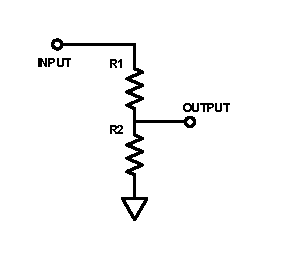
\includegraphics{images/plot2.pdf}
    %     \caption{A voltage divider}
    %     \label{fig:2}
    % \end{figure}

    % \begin{table}[h]
    % \begin{ruledtabular}
    % \begin{tabular}{cccc} 
    % Load[k$\Omega$] &  Output Voltage[V] & $R_\text{th}[\Omega]$ & Theoretical Voltage\\ \hline\hline
    % 50              & 0.680(1)           & 501(1)                & 0.682 \\ \hline
    % 500             & 3.75(1)            & 500(1)                & 3.75 \\ \hline
    % 5000            & 6.80(1)            & 514(1)                & 6.82 \\
    % \end{tabular}
    % \end{ruledtabular}
    % \caption{Load resistor and the output}
    % \label{table:8}
    % \end{table} 

% \begin{center}
%  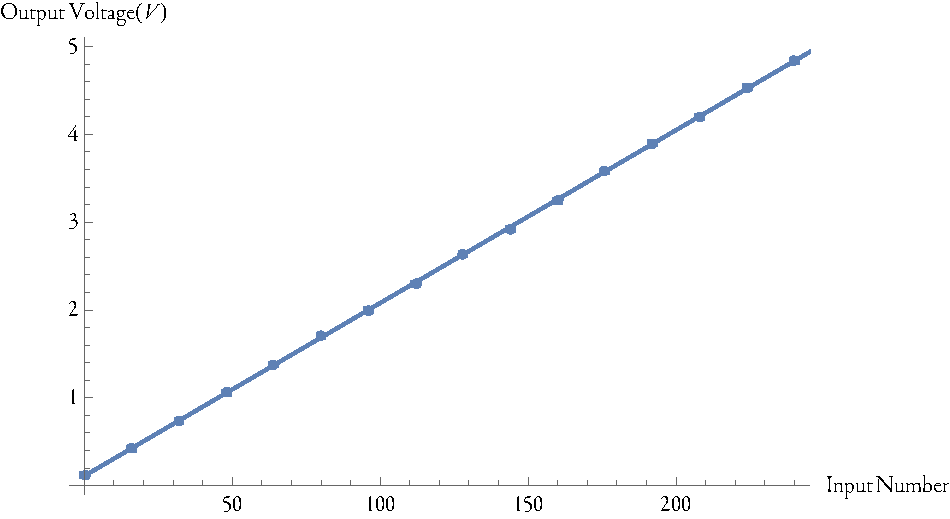
\includegraphics[height=1.8in]{plot.pdf}
% \end{center} 

%\begin{center}
% 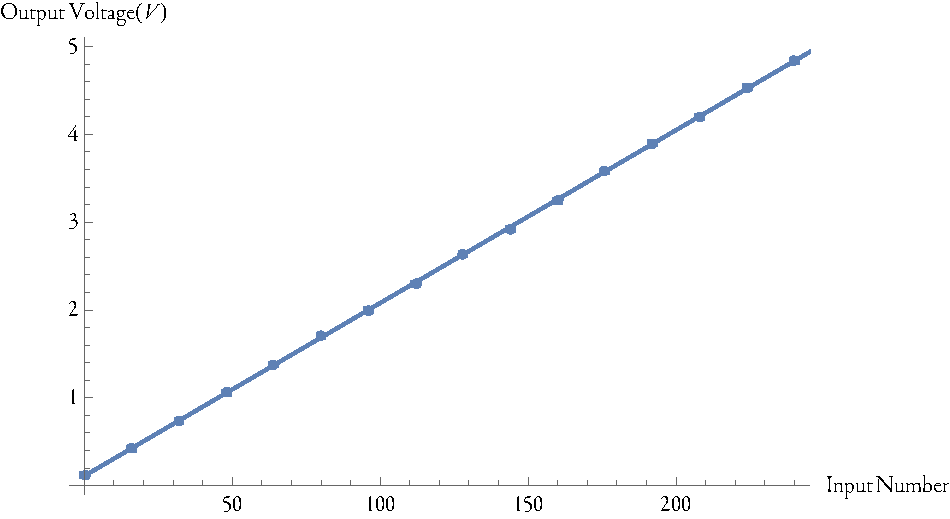
\includegraphics[height=1.3in]{plot.pdf}
%\end{center}

% \blindtext \cite{article-minimal}

% \bibliographystyle{apsrev4-1} % Tell bibtex which bibliography style to use
% \bibliography{xampl} % Tell bibtex which .bib file to use (this one is some example file in TexLive's file tree)

\end{document}